% !TeX program = pdflatex
% Architecture Documentation: Standards, Frameworks, Modeling Languages, and Tooling
% Self-contained technical handout. Compile with: latexmk -pdf -interaction=nonstopmode <file>.tex
\documentclass[11pt,letterpaper,oneside]{article}
\usepackage[letterpaper,margin=0.83in,headheight=16pt,headsep=19pt,footskip=28pt]{geometry}
\usepackage[T1]{fontenc}
\usepackage[utf8]{inputenc}
\usepackage{lmodern}
\usepackage{microtype}
\usepackage{amsmath,amssymb}
\usepackage{array,booktabs,tabularx,longtable,multirow}
\usepackage[table]{xcolor}
\usepackage{graphicx}
\usepackage{tikz}
\usetikzlibrary{arrows.meta,positioning,calc,fit,shapes.geometric}
\usepackage{tcolorbox}
\tcbuselibrary{skins,breakable}
\usepackage{enumitem}
\usepackage{titlesec}
\usepackage{fancyhdr}
\usepackage{hyperref}
\usepackage{listings}
\usepackage{caption}
\usepackage{needspace}
\usepackage{etoolbox}
\usepackage{ragged2e}
\usepackage{lastpage}
\usepackage{url}
\usepackage{parskip}

% Design system
\definecolor{Navy}{HTML}{14283D}
\definecolor{Ink}{HTML}{263646}
\definecolor{Teal}{HTML}{047E8C}
\definecolor{Sky}{HTML}{EDF6F8}
\definecolor{Slate}{HTML}{64788C}
\definecolor{Border}{HTML}{D5E1E6}
\definecolor{Mist}{HTML}{F5F8FA}
\definecolor{LightTeal}{HTML}{D7EDF0}
\definecolor{Gold}{HTML}{B47B25}
\color{Ink}

\hypersetup{
  colorlinks=true,
  linkcolor=Teal,
  urlcolor=Teal,
  citecolor=Teal,
  pdftitle={Architecture Documentation: Standards, Frameworks, Modeling Languages, and Tooling},
  pdfsubject={Technical reference and architectural documentation strategy},
  pdfkeywords={ISO 42010, Views and Beyond, C4, UML, PlantUML, architecture documentation},
  pdfauthor={Architecture Engineering Technical Reference}
}
\urlstyle{same}
\setlength{\parindent}{0pt}
\setlength{\parskip}{6pt plus 2pt minus 1pt}
\emergencystretch=2em
\renewcommand{\arraystretch}{1.23}
\setlist[itemize]{leftmargin=1.3em,topsep=3pt,itemsep=2pt,parsep=0pt}
\setlist[enumerate]{leftmargin=1.45em,topsep=4pt,itemsep=3pt,parsep=0pt}
\titleformat{\section}{\Large\bfseries\color{Navy}}{\thesection}{0.75em}{}
\titleformat{\subsection}{\large\bfseries\color{Teal}}{\thesubsection}{0.7em}{}
\titleformat{\subsubsection}{\normalsize\bfseries\color{Navy}}{\thesubsubsection}{0.7em}{}
\titlespacing*{\section}{0pt}{23pt}{10pt}
\titlespacing*{\subsection}{0pt}{16pt}{6pt}
\titlespacing*{\subsubsection}{0pt}{11pt}{4pt}
\pretocmd{\section}{\Needspace{6\baselineskip}}{}{}
\pretocmd{\subsection}{\Needspace{4\baselineskip}}{}{}
\captionsetup{font=small,labelfont={bf,color=Navy},textfont={color=Slate},skip=7pt}

\pagestyle{fancy}
\fancyhf{}
\fancyhead[L]{\footnotesize\bfseries\color{Navy} ARCHITECTURE ENGINEERING}
\fancyhead[R]{\footnotesize\color{Slate} TECHNICAL REFERENCE  /  2026}
\fancyfoot[L]{\footnotesize\color{Slate} Standards \textbullet\ Frameworks \textbullet\ Modeling \textbullet\ Tooling}
\fancyfoot[R]{\footnotesize\color{Slate} \thepage\ / \pageref{LastPage}}
\renewcommand{\headrulewidth}{0.35pt}
\renewcommand{\footrulewidth}{0pt}

\newtcolorbox{keybox}[1][]{enhanced,breakable,colback=Sky,colframe=Border,boxrule=0.65pt,
  arc=2mm,left=11pt,right=11pt,top=9pt,bottom=9pt,borderline west={3pt}{0pt}{Teal},#1}
\newtcolorbox{notebox}[1][]{enhanced,breakable,colback=Mist,colframe=Border,boxrule=0.55pt,
  arc=1.5mm,left=10pt,right=10pt,top=8pt,bottom=8pt,#1}
\newcommand{\term}[1]{\textbf{\color{Navy}#1}}
\newcommand{\pill}[1]{\colorbox{LightTeal}{\strut\scriptsize\bfseries\color{Navy}\ #1\ }}
\newcolumntype{L}[1]{>{\RaggedRight\arraybackslash}p{#1}}
\newcolumntype{Y}{>{\RaggedRight\arraybackslash}X}
\newcommand{\thead}[1]{\textcolor{white}{\bfseries #1}}

\lstdefinestyle{archcode}{
 basicstyle=\ttfamily\footnotesize,
 keywordstyle=\color{Teal}\bfseries,
 commentstyle=\color{Slate}\itshape,
 stringstyle=\color{Navy},
 backgroundcolor=\color{Mist},
 frame=single,rulecolor=\color{Border},
 framerule=0.5pt,
 xleftmargin=0.2em,xrightmargin=0.2em,
 framexleftmargin=0.85em,framexrightmargin=0.8em,
 aboveskip=9pt,belowskip=9pt,
 breaklines=true,showstringspaces=false,
 columns=fullflexible,keepspaces=true,
 morekeywords={Person,System,System_Boundary,Container,ContainerDb,Rel,LAYOUT_LEFT_RIGHT,SHOW_LEGEND}
}

\begin{document}
\thispagestyle{empty}
\vspace*{0.42in}
\begin{tikzpicture}[remember picture,overlay]
  \fill[Navy] (current page.north west) rectangle ([yshift=-0.22in]current page.north east);
  \fill[Teal] ([yshift=-0.22in]current page.north west) rectangle ([yshift=-0.29in]current page.north east);
\end{tikzpicture}
\vspace{0.32in}
{\small\bfseries\color{Teal}\MakeUppercase{Software Architecture / Technical Reference}}\par
\vspace{0.24in}
{\fontsize{31}{36}\selectfont\bfseries\color{Navy} Architecture\par Documentation}\par
\vspace{0.17in}
{\Large\color{Slate} Standards, Frameworks, Modeling Languages,\par and Tooling}\par
\vspace{0.34in}
\rule{\textwidth}{0.8pt}
\vspace{0.20in}
{\large\bfseries\color{Navy}ISO/IEC/IEEE 42010:2022\par
Views and Beyond \quad\textbullet\quad C4 Model\par
UML 2.5.1 \quad\textbullet\quad PlantUML}\par
\vspace{0.38in}
\begin{keybox}
\textbf{Central thesis.} These are complementary responsibilities within an architecture documentation practice, not a mandatory linear technology stack. A standard defines description obligations; approaches help select and structure views; modeling languages express selected models; tools generate and manage artifacts. The quality of the result depends on stakeholder coverage, consistency, rationale, and review---not on diagram rendering alone.
\end{keybox}
\vfill
\begin{tabularx}{\textwidth}{@{}L{0.30\textwidth}Y@{}}
\textbf{Document type} & Architecture documentation strategy and comparative technical reference\\
\textbf{Intended audience} & Software architects, engineering leads, platform teams, and architecture governance practitioners\\
\textbf{Version / date} & 1.0 \quad/\quad 29 October 2026\\
\textbf{Scope} & Conceptual alignment, pragmatic selection, documentation artifacts, and automated validation\\
\end{tabularx}
\vspace{0.10in}
\clearpage

\tableofcontents
\vspace{0.25in}
\begin{notebox}
\textbf{Reading guide.} Sections \ref{sec:landscape}--\ref{sec:crosswalk} establish the conceptual distinctions; Sections \ref{sec:artifacts}--\ref{sec:implementation} translate them into an operational documentation strategy. The crosswalks describe useful correspondences, not standards-mandated mappings.
\end{notebox}
\clearpage

\section{Executive summary}\label{sec:summary}
A practical learning sequence is often:
\begin{center}
\textbf{ISO/IEC/IEEE 42010:2022 $\rightarrow$ Views and Beyond $\rightarrow$ C4 $\rightarrow$ UML $\rightarrow$ PlantUML.}
\end{center}
This sequence proceeds from principles of architecture description toward concrete visual output. It is \emph{pedagogically useful}, but it does not imply a formal dependency chain. Each item addresses a different design or documentation decision.

\begin{keybox}
\textbf{Recommended engineering model}\par
\textbf{Description requirements} $\rightarrow$ \textbf{Stakeholder concerns and viewpoints} $\rightarrow$ \textbf{Views and models} $\rightarrow$ \textbf{Notations} $\rightarrow$ \textbf{Authoring and rendering tools} $\rightarrow$ \textbf{Review and validation}.
\end{keybox}

Five governing principles follow:
\begin{enumerate}[label=\arabic*.]
\item \textbf{Keep the architecture distinct from its description.} The system architecture exists regardless of how it is documented; an architecture description (AD) expresses it for stakeholders. ISO/IEC/IEEE 42010:2022 defines requirements for ADs and related description constructs, not for the architecture itself \cite{iso42010}.
\item \textbf{Select views by concern, not by diagram quota.} Views and Beyond starts from what stakeholders need to understand; its three fundamental viewtypes help expose different kinds of system structure \cite{viewsbeyond,sei}. 
\item \textbf{Use C4 as an effective communication vocabulary.} C4 supplies hierarchical structural views and additional dynamic, deployment, and landscape diagrams; not all diagram levels are necessary \cite{c4diagrams}.
\item \textbf{Employ UML when semantics justify it.} UML models structures and behaviors and is not limited to a C4 Code diagram \cite{uml}.
\item \textbf{Separate rendering from assurance.} PlantUML and C4-PlantUML turn text into diagrams, but a successful rendering does not establish architectural completeness, traceability, or standards conformance \cite{plantuml,c4plantuml}.
\end{enumerate}

\section{Positioning the five concepts}\label{sec:landscape}
\small
\rowcolors{2}{Mist}{white}
\begin{tabularx}{\textwidth}{@{}L{0.22\textwidth}L{0.20\textwidth}Y@{}}
\rowcolor{Navy}\thead{Concept} & \thead{Category} & \thead{Primary responsibility}\\
ISO/IEC/IEEE 42010:2022 & International standard & Requirements and concepts for architecture descriptions, architecture viewpoints, views, model kinds, and related description elements.\\
Views and Beyond & Documentation approach & Selects and documents relevant module, component-and-connector, and allocation structures.\\
C4 Model & Visualization approach & Communicates software architecture through context, container, component, and optional code views, with supporting diagram types.\\
UML 2.5.1 & Modeling language & Formalizes structural and behavioral modeling constructs and their semantics.\\
PlantUML / C4-PlantUML & Diagram-as-code tooling & Renders textual diagram definitions; C4-PlantUML contributes C4-specific macros and conventions.\\
\end{tabularx}
\normalsize
\vspace{0.13in}
\begin{notebox}
\textbf{Terminological precision.} Calling Views and Beyond or C4 an \emph{ISO 42010 architecture description framework} without establishing applicable framework requirements would overstate the relationship. They are useful methods or approaches that may inform an AD. Likewise, UML is a modeling language, while PlantUML is principally a textual diagramming tool; generating a diagram is not the same as verifying full UML semantics.
\end{notebox}

\section{Conceptual integration model}\label{sec:model}
Figure~\ref{fig:integration} illustrates the practical connection between governance, architecture communication, notation, and tooling. The parallel boxes show that Views and Beyond and C4 can be adopted together or separately.

\begin{figure}[htbp]
\centering
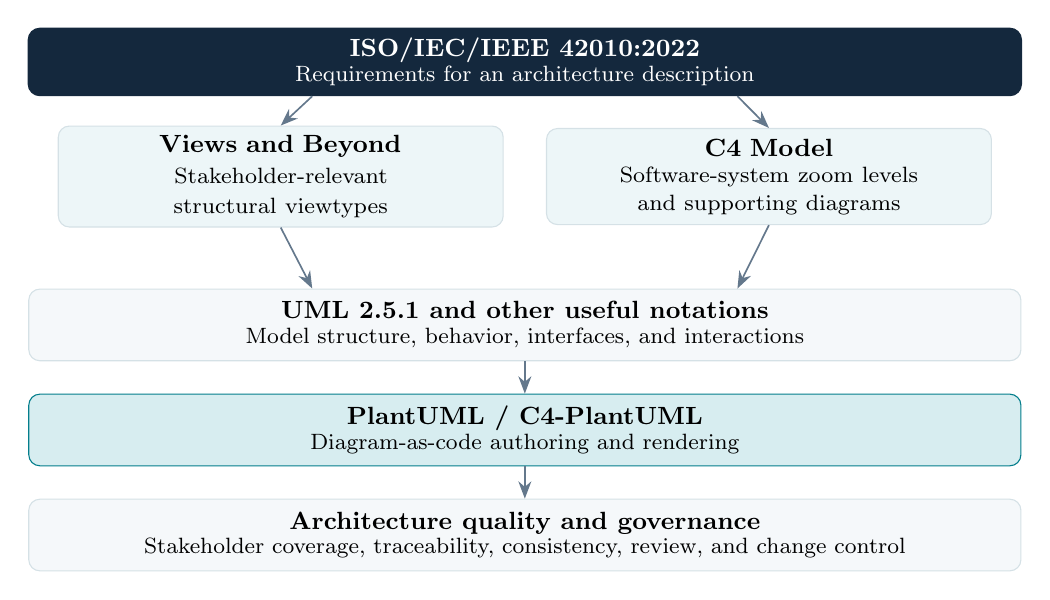
\begin{tikzpicture}[
  font=\small,
  top/.style={draw=Navy,fill=Navy,text=white,thick,rounded corners=4pt,minimum width=12.6cm,minimum height=0.78cm,align=center},
  approach/.style={draw=Border,fill=Sky,rounded corners=4pt,text width=5.35cm,minimum width=5.65cm,minimum height=1.22cm,align=center},
  layer/.style={draw=Border,fill=Mist,rounded corners=4pt,minimum width=12.6cm,minimum height=0.91cm,align=center},
  tool/.style={draw=Teal,fill=LightTeal,rounded corners=4pt,minimum width=12.6cm,minimum height=0.91cm,align=center},
  arr/.style={-{Stealth[length=2.2mm]},semithick,draw=Slate}
]
\node[top] (iso) {\textbf{ISO/IEC/IEEE 42010:2022}\\[-2pt]\footnotesize Requirements for an architecture description};
\node[approach] (vb) at ($(iso.south)+(-3.10cm,-1.02cm)$) {\textbf{Views and Beyond}\\\footnotesize Stakeholder-relevant structural viewtypes};
\node[approach] (c4) at ($(iso.south)+(3.10cm,-1.02cm)$) {\textbf{C4 Model}\\\footnotesize Software-system zoom levels\\[-1pt]\footnotesize and supporting diagrams};
\node[layer,below=0.79cm of $(vb.south)!0.5!(c4.south)$] (notation) {\textbf{UML 2.5.1 and other useful notations}\\[-2pt]\footnotesize Model structure, behavior, interfaces, and interactions};
\node[tool,below=0.41cm of notation] (tooling) {\textbf{PlantUML / C4-PlantUML}\\[-2pt]\footnotesize Diagram-as-code authoring and rendering};
\node[layer,below=0.41cm of tooling] (qa) {\textbf{Architecture quality and governance}\\[-2pt]\footnotesize Stakeholder coverage, traceability, consistency, review, and change control};
\draw[arr] ([xshift=-2.7cm]iso.south) -- (vb.north);
\draw[arr] ([xshift=2.7cm]iso.south) -- (c4.north);
\draw[arr] (vb.south) -- ([xshift=-2.7cm]notation.north);
\draw[arr] (c4.south) -- ([xshift=2.7cm]notation.north);
\draw[arr] (notation) -- (tooling);
\draw[arr] (tooling) -- (qa);
\end{tikzpicture}
\caption{Practical integration of standards, documentation approaches, modeling, tooling, and assurance. This is an illustrative engineering model, not an ISO-prescribed process or dependency chain.}
\label{fig:integration}
\end{figure}

\subsection{Why Views and Beyond may precede C4 in a curriculum}
Views and Beyond provides an extensive vocabulary for reasoning about implementation units, runtime interactions, and mapping software to environments. Learning these distinctions first can make later C4 diagrams more intentional. C4 then supplies a concise, developer-oriented way to communicate selected perspectives. The ordering is an instructional preference, not a requirement imposed by either approach \cite{viewsbeyond,c4home}.

\subsection{Why UML is not simply the last C4 zoom level}
A UML sequence diagram may explain interactions visible at a C4 Container or Component level; a UML deployment diagram may complement a C4 Deployment diagram; and package or component diagrams may clarify static dependencies. UML class diagrams can be useful at the Code level, but UML has a wider application than that single level \cite{uml,c4intro}.

\section{Architecture view crosswalk}\label{sec:crosswalk}
\rowcolors{2}{Mist}{white}
\small
\begin{tabularx}{\textwidth}{@{}L{0.18\textwidth}L{0.24\textwidth}L{0.24\textwidth}Y@{}}
\rowcolor{Navy}\thead{Concern} & \thead{Views and Beyond} & \thead{C4 view} & \thead{Potential UML notation}\\
System boundary, users, external dependencies & Context documentation alongside relevant views & System Context; System Landscape & Use Case\\
Implementation decomposition & Module viewtype & Container; Component & Package; Component\\
Runtime elements and connectors & Component-and-Connector viewtype & Container; Dynamic & Sequence; Communication\\
Deployment and environment mapping & Allocation viewtype & Deployment & Deployment\\
Code-level structure & Module viewtype & Optional Code & Class; Package\\
Behavior and workflows & Behavioral documentation related to selected views & Dynamic and other supporting views & Activity; State Machine; Sequence\\
\end{tabularx}
\normalsize

\begin{keybox}
\textbf{Reading the crosswalk correctly.} A row indicates that the techniques can address overlapping stakeholder questions. It does \emph{not} assert formal equivalence between V\&B viewtypes, C4 diagram types, or UML diagrams. In particular, the word \emph{component} does not guarantee the same meaning across methods.
\end{keybox}

\subsection{C4 diagram selection rule}
Start with System Context and Container diagrams when they answer the architectural questions at hand. Add Component diagrams for areas that materially benefit from greater detail; include Code diagrams when they are useful and maintainable, preferably generated or constrained to stable areas. Consider Dynamic and Deployment diagrams where runtime sequences or hosting topology need explicit treatment \cite{c4diagrams,c4faq}.

\section{Architecture artifacts and traceability}\label{sec:artifacts}
Document families should be classified by \emph{their purpose}, not simply by whether they contain a diagram. The following distinctions support consistent storage, review, and lifecycle management.

\rowcolors{2}{Mist}{white}
\small
\begin{tabularx}{\textwidth}{@{}L{0.25\textwidth}Y L{0.20\textwidth}@{}}
\rowcolor{Navy}\thead{Artifact family} & \thead{Primary question} & \thead{Typical contents}\\
Architecture Description (AD) & How is the architecture expressed as a coherent set of stakeholder-relevant information? & Scope, concerns, views, models, rationale, correspondences\\
Architecture Viewpoint Specification (AVS) & How should a view addressing a particular concern be constructed and interpreted? & Purpose, stakeholders, concerns, model kinds, conventions, checks\\
Architecture View / Model & What structural or behavioral aspect is represented? & Diagrams, model elements, relationships, explanations, assumptions\\
Architecture Decision Record (ADR) & Why was a significant architectural choice made? & Context, drivers, options, decision, consequences, status\\
Architecture Scorecard / Assessment & How well does the documented architecture address expected qualities? & Criteria, evidence, ratings, findings, actions\\
\end{tabularx}
\normalsize

\subsection{Suggested traceability chain}
\begin{center}
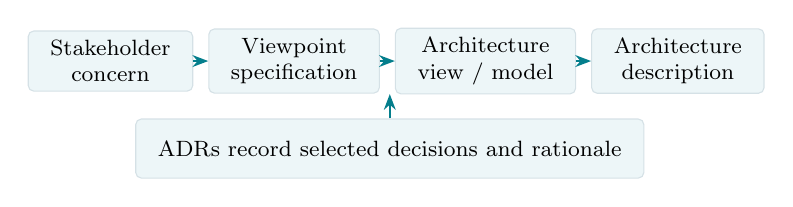
\begin{tikzpicture}[node distance=0.19cm,font=\footnotesize,
 n/.style={draw=Border,fill=Sky,rounded corners=2pt,minimum height=0.75cm,align=center,inner xsep=8pt},
 a/.style={-{Stealth[length=2mm]},draw=Teal,thick}]
\node[n] (s) {Stakeholder\\concern};
\node[n,right=of s] (v) {Viewpoint\\specification};
\node[n,right=of v] (m) {Architecture\\view / model};
\node[n,right=of m] (ad) {Architecture\\description};
\draw[a] (s)--(v); \draw[a] (v)--(m); \draw[a] (m)--(ad);
\node[n,below=0.31cm of $(v.south)!0.5!(m.south)$] (adr) {ADRs record selected decisions and rationale};
\draw[a] (adr.north)--($(v.south)!0.5!(m.south)$);
\end{tikzpicture}
\end{center}
The chain above is a proposed repository traceability convention, not a one-to-one relationship mandated by the standard. Views, model kinds, decisions, and evidence may have many-to-many relationships; stable identifiers help preserve them across revisions.

\subsection{Template--Blank lifecycle}
For reusable documentation repositories, maintain \term{Template} and \term{Blank} as distinct deliverables where both are needed:
\begin{itemize}
\item \textbf{Template:} explanatory prompts, examples, completion rules, section intent, and validation guidance.
\item \textbf{Blank:} the same operative structure with printable empty fields or writing areas; no instructional placeholders such as \texttt{[To complete]}.
\item \textbf{Completed record:} a project- or system-specific instance, with provenance, owner, revision history, and appropriate review status.
\end{itemize}
The Template--Blank distinction is a recommended document-control practice, not an ISO 42010 conformance condition.

\section{Putting the strategy into practice}\label{sec:implementation}
\subsection{A concern-driven workflow}
\begin{enumerate}[label=\textbf{Step \arabic*.}]
\item \textbf{Define scope and identify stakeholders.} Establish the entity of interest, system boundary, users, operators, governance roles, and the decisions the documentation must support.
\item \textbf{Record architecture concerns.} Capture security boundaries, reliability, modifiability, data ownership, runtime behavior, deployment, or other questions that require architectural evidence.
\item \textbf{Select and specify viewpoints.} Record the intended audience, concerns addressed, model kinds, notation, assumptions, and consistency expectations.
\item \textbf{Choose meaningful views.} Draw on V\&B structural viewtypes and C4 diagram levels as appropriate; do not generate diagrams without a stated use.
\item \textbf{Apply precision only where justified.} Add UML or another modeling language when the required semantics cannot be communicated adequately by simpler diagrams.
\item \textbf{Generate, integrate, and reference artifacts.} Render source-controlled diagrams and embed them in the AD; connect important architectural decisions to relevant views.
\item \textbf{Validate and review.} Verify syntax, diagram output, naming consistency, cross-view correspondence, ownership, stakeholder coverage, and evidence traceability.
\end{enumerate}

\subsection{Example: C4-PlantUML as a rendering input}
The example below is a small, self-contained C4-PlantUML \emph{source snippet} for an illustrative software system. It uses the standard-library C4 include supported by PlantUML installations that bundle the C4 library \cite{c4plantuml}. It is shown for tooling context; the LaTeX document itself does not require PlantUML to compile.
\begin{lstlisting}[style=archcode,language={},caption={Example source file: \texttt{diagrams/system-container.puml}}]
@startuml
!include <C4/C4_Container>
LAYOUT_LEFT_RIGHT()

Person(operator, "Operator", "Uses the service")
System_Boundary(s1, "Order Service") {
  Container(api, "Order API", "Java", "Request handling")
  ContainerDb(store, "Orders DB", "PostgreSQL", "Order records")
}
Rel(operator, api, "Submits requests", "HTTPS")
Rel(api, store, "Reads/writes", "SQL")
SHOW_LEGEND()
@enduml
\end{lstlisting}

\begin{lstlisting}[style=archcode,language={},caption={Illustrative local build commands}]
# Generate a vector diagram; no network dependency required
# when the local PlantUML distribution includes C4.
plantuml -tsvg diagrams/system-container.puml

# Build the LaTeX technical reference.
latexmk -pdf -interaction=nonstopmode architecture-reference.tex
\end{lstlisting}

\subsection{Suggested source-controlled repository structure}
\begin{lstlisting}[style=archcode,language={},caption={Illustrative artifact taxonomy, not a required standard layout}]
architecture/
  technical-references/
    standards-frameworks-and-tooling.tex
  descriptions/
    templates/
    blanks/
    completed/
  viewpoints/
    templates/
    blanks/
    specifications/
  decisions/
    templates/
    blanks/
    records/
  diagrams/
    c4/
    uml/
  assessments/
    templates/
    blanks/
\end{lstlisting}
\begin{notebox}
\textbf{Reproducibility.} Prefer pinned diagram-tool versions, locally vendored diagram libraries where necessary, stable artifact identifiers, automated builds, and a policy against manually editing generated images. PDF and SVG outputs should be treated as build artifacts derived from reviewable sources.
\end{notebox}

\section{Verification and governance criteria}\label{sec:governance}
Diagram rendering is the first check, not the last. A mature practice distinguishes multiple quality gates.
\small
\rowcolors{2}{Mist}{white}
\begin{tabularx}{\textwidth}{@{}L{0.23\textwidth}Y L{0.25\textwidth}@{}}
\rowcolor{Navy}\thead{Quality gate} & \thead{Validation objective} & \thead{Example evidence}\\
Source quality & Files parse, dependencies resolve, repeatable builds succeed & CI job, build log\\
Visual integrity & Labels remain legible; relationships and boundaries are unambiguous & Render review, diagram lint\\
Semantic consistency & Names, identifiers, and relationships agree across diagrams & Cross-reference checks\\
Concern coverage & Each priority stakeholder concern is addressed by suitable documentation & Concern-to-view matrix\\
Decision traceability & Important choices and consequences connect to affected architectural elements & ADR identifiers and links\\
Currency and ownership & Changes are reviewed and stale documents are identified & Owners, revisions, review dates\\
Conformance claims & Any asserted standard conformance has an explicit basis and scope & Controlled conformance review\\
\end{tabularx}
\normalsize

\subsection{A minimum architecture-documentation checklist}
\begin{itemize}[label=$\square$]
\item Defined entity of interest, scope, and relevant system context.
\item Named stakeholder groups and their documented architectural concerns.
\item Selected viewpoints with clear purpose and applicable modeling conventions.
\item Architecture views and models that answer those concerns.
\item Consistent element naming, boundaries, and relationships across views.
\item Documented significant decisions and rationale, with cross-references.
\item Reproducible diagram generation and validated document builds.
\item Review owner, change history, and a procedure for keeping artifacts current.
\end{itemize}

\section{Decision guidance and final recommendation}\label{sec:recommend}
\begin{keybox}
\textbf{Recommended reference architecture for documentation engineering}\par
Use \term{ISO/IEC/IEEE 42010:2022} as the reference for architecture-description requirements; apply \term{Views and Beyond} to reason about necessary structural views; use \term{C4} for approachable software-architecture communication; use \term{UML} selectively when stronger modeling semantics are warranted; employ \term{PlantUML/C4-PlantUML} to generate maintainable, text-based diagrams; and operate the entire system under \term{independent quality, traceability, and governance controls}.
\end{keybox}

This strategy deliberately separates \emph{what must be described}, \emph{which concerns motivate it}, \emph{how to represent it}, and \emph{how the representations are produced and checked}. The resulting architecture documentation is both accessible to engineering teams and more defensible in formal reviews.

For learning, the five-item sequence remains sound as an instructional pathway. For architecture governance, the more accurate sequence is concern-driven and iterative: \textbf{requirements $\rightarrow$ viewpoints $\rightarrow$ views/models $\rightarrow$ notation $\rightarrow$ tooling $\rightarrow$ validation}. The cycle returns to stakeholder concerns whenever a review reveals omissions, discrepancies, or evolving requirements.

\subsection{Selection patterns for different engineering contexts}
\small
\rowcolors{2}{Mist}{white}
\begin{tabularx}{\textwidth}{@{}L{0.24\textwidth}Y@{}}
\rowcolor{Navy}\thead{Engineering context} & \thead{Practical documentation baseline}\\
Small service or product team & A concise AD, C4 System Context and Container diagrams, and ADRs for consequential architectural choices. Expand detail only when a stakeholder concern warrants it.\\
Distributed platform or microservices & Include runtime interactions, ownership and deployment boundaries, selected C\&C perspectives, C4 Dynamic or Deployment diagrams, and UML sequence diagrams for critical flows.\\
Regulated or high-assurance environment & Define explicit viewpoint specifications, trace concerns to architecture evidence, review cross-view consistency, retain decisions and approvals, and separately evaluate any formal conformance claims.\\
Legacy modernization or migration & Describe as-is and target-state structures, record architectural constraints and assumptions, show transition dependencies, and track migration decisions through ADRs and traceability links.\\
\end{tabularx}
\normalsize

\begin{notebox}
\textbf{Operational acceptance criterion.} Documentation is ready for use when a reviewer can locate the applicable stakeholder concern, find the view or model addressing it, understand the decisions shaping it, and reproduce the published representations from version-controlled sources.
\end{notebox}

\clearpage
\section{References and source authority}\label{sec:references}
\begin{thebibliography}{9}
\setlength{\itemsep}{7pt}
\bibitem{iso42010} ISO/IEC/IEEE. \emph{ISO/IEC/IEEE 42010:2022: Software, systems and enterprise---Architecture description}. Second edition, November 2022. Official standard overview: \url{https://www.iso.org/standard/74393.html}.

\bibitem{viewsbeyond} Clements, P., et al. \emph{Documenting Software Architectures: Views and Beyond}. Second edition, Addison-Wesley, published 2010 (copyright 2011). Publisher description and table of contents: \url{https://www.informit.com/store/documenting-software-architectures-views-and-beyond-9780132488594}.

\bibitem{sei} Software Engineering Institute, Carnegie Mellon University. \emph{Documenting Software Architectures: A Hands-on Introduction}. SEI Technical Report CMU/SEI-2004-TR-008. \url{https://resources.sei.cmu.edu/asset_files/TechnicalReport/2004_005_001_14387.pdf}.

\bibitem{c4home} Brown, S. \emph{The C4 Model for Visualising Software Architecture}. Official introduction: \url{https://c4model.com/}.

\bibitem{c4diagrams} Brown, S. \emph{The C4 Model: Diagrams}. Official guidance: \url{https://c4model.com/diagrams}.

\bibitem{c4faq} Brown, S. \emph{The C4 Model: Diagram FAQ}. Official maintenance guidance: \url{https://c4model.com/diagrams/faq}.

\bibitem{c4intro} Brown, S. \emph{The C4 Model: Introduction}. Official explanation of zoom levels and notation: \url{https://c4model.com/introduction}.

\bibitem{uml} Object Management Group. \emph{Unified Modeling Language (UML), Version 2.5.1}. December 2017. Official specification: \url{https://www.omg.org/spec/UML/2.5.1}.

\bibitem{plantuml} PlantUML. \emph{PlantUML Documentation}. Official project: \url{https://plantuml.com/}.

\bibitem{c4plantuml} C4-PlantUML contributors. \emph{C4-PlantUML: PlantUML Macros for C4 Diagrams}. Official open-source project: \url{https://github.com/plantuml-stdlib/C4-PlantUML}.
\end{thebibliography}

\vspace{0.16in}
\begin{notebox}
\small\textbf{Scope and attribution note.} This handout synthesizes primary standards descriptions and official documentation. It is not a substitute for the licensed full text of ISO/IEC/IEEE 42010:2022, nor does it assert formal conformance on behalf of any architecture description, framework, modeling language, or tool.
\end{notebox}

\end{document}
